\documentclass[10pt]{amsart}

\usepackage{algorithm}
\usepackage[noend]{algpseudocode}
\usepackage{amsfonts}
\usepackage{amsmath}
\usepackage{amssymb}
\usepackage{amsthm}
\usepackage[backend=biber, citestyle=numeric-comp, bibstyle=ieee]{biblatex}
\usepackage{changepage}
\usepackage{enumitem}
\usepackage{fancyhdr}
\usepackage{fontspec}
\usepackage{fullpage}
\usepackage[hidelinks]{hyperref}
\usepackage{marvosym}
\usepackage{mathtools}
\usepackage[]{mdframed}
\usepackage{physics}
\usepackage{thmtools}
\usepackage{tikz}
\usepackage{tikz-3dplot}
\usetikzlibrary{angles, cd, quantikz, quotes, patterns}
\usepackage{titlesec}
\usepackage{wasysym}

\usepackage{tikz-cd}

\usepackage{bookmark}
\usepackage[nameinlink]{cleveref}

\titleformat{\section}{\normalsize\bfseries}{\thesection}{1em}{}
\titleformat{\subsection}{\normalsize\bfseries}{\thesubsection}{1em}{}
\titleformat{\subsubsection}{\normalsize\bfseries}{\thesubsubsection}{1em}{}

\addbibresource{mts_and_wfa_notes.bib}

\theoremstyle{definition}
\newtheorem{theorem}{Theorem}
\newtheorem{conjecture}{Conjecture}
\newtheorem{definition}{Definition}
\theoremstyle{remark}
\newtheorem{problem}[theorem]{Problem}
\newtheorem{lemma}[theorem]{Lemma}
\newtheorem{remark}[theorem]{Remark}
\newtheorem{observation}[theorem]{Observation}
\newtheorem{example}[theorem]{Example}
\newtheorem{corollary}[theorem]{Corollary}

\renewcommand{\qedsymbol}{\(\blacksquare\)}

\setlength{\parindent}{0pt}

\DeclareMathOperator{\controrot}{CR}
\DeclareMathOperator{\expectation}{E}
\DeclareMathOperator{\gf}{GF}
\DeclareMathOperator{\qft}{QFT}
\DeclareMathOperator{\rk}{rk}
\DeclareMathOperator{\defect}{def}
\DeclareMathOperator{\swapgate}{SWAP}
\DeclareMathOperator{\che}{CHE}
\DeclareMathOperator{\poly}{poly}
\DeclareMathOperator{\Span}{Span}
\DeclareMathOperator{\diag}{diag}

\newcommand{\djk}{\delta_{j, k}}
\newcommand{\tlk}{\tilde{\lambda_k}}

\newcommand{\evalat}[2]{\left.{#1}\middle|\right._{#2}}

% SOURCE: https://tex.stackexchange.com/questions/296151/double-head-and-hook-arrow
\newcommand{\hookdoubleheadrightarrow}{%
  \hookrightarrow\mathrel{\mspace{-15mu}}\rightarrow
}

\AtEveryBibitem{%
  \clearfield{journaltitle}%
  \clearfield{date}%
  \clearfield{volume}%
  \clearfield{pages}%
  \clearfield{publisher}%
  \clearfield{number}%
  \clearfield{journaltitle}%
}

\begin{document}
    %noty notes

    %\begin{itemize}
    %    \item Metrical Task Systems model online algorithms in a general framework and allow for a weak competitive analysis. Formulated by Borodin, Linial and Saks.
    %    \item Perhaps: Present MTS formulations for a couple of problems, select them.
    %    \item Most interesting aspect perhaps: Work function algorithm. How good? Optimal for which problems, for which not and for which unknown?
    %    \item Proof for competitiveness of work function algorithm perhaps? Surely depends on difficulty of proof.
    %    \item There seems to be a lot of info about the connection to \(k\)-server. That would intersect with the \(k\)-server topic, wouldn't it? \(\rightarrow\) I would actually like to do something different than \(k\)-server, is there anything? I have looked online and there are some things like some graph theoretic results or Ramsey-type theorems, but they are mostly based on the randomized model.
    %    \item Is this citation style alright for Laszlo? \(\rightarrow\) It's fine.
    %    \item I think the books contain enough info for the presentation, to be honest. I may research some articles for recent major results, if there are any.
    %    \item Probably include the \(2N-1\) WFA algorithm with lower bound.
    %    \item \cite{Buchbinder2009} is not a good source, as the whole chapter there is based on the continuous MTS model and utilizes linear programming.
    %    \item There seem to be very strong results on randomized algorithms for MSTs: \url{https://arxiv.org/abs/1904.03874v1}. There is also a result in the book by Borodin and El-Yaniv for \(2\ln(N+1)\)-competitiveness. Maybe just mention them at the end of presentation. Also mention hierarchical aspects.
    %    \item Special cases of \(k\)-server, general paging is lower competitive.
    %\end{itemize}

    %\newpage

    \begin{mdframed}
        \textsc{Seminar on Online Algorithms} \hfill valentinpi\\
        Freie Universität Berlin \hfill May 2, 2023\\
        Summer Term 2023
    \end{mdframed}

    \phantom{}

    \textbf{Presentation Notes on: Metrical Task Systems and the Work Function Algorithm}

    We present an abstract model for the competitive analysis of online algorithms, discuss a general solution algorithm and state some bounds for specific problems.

    \phantom{}

    \paragraph{\textbf{Preliminaries}} We shall first recall the definition of a metric.

    \begin{definition}[{\cite[pp. 3-4]{Forster2017}}]
        Let \(\mathcal{M}\) be a set. A \emph{metric} is a map \(d\colon \mathcal{M} \times \mathcal{M} \to \mathbb{R}\) with the following properties for any \(x, y, z \in \mathcal{M}\):
        \begin{enumerate}[label=(\roman*)]
            \item \(d(x, y) = 0 \leftrightarrow x = y\)
            \item \(d(x, y) = d(y, x)\) (Symmetry)
            \item \(d(x, z) \leq d(x, y) + d(y, z)\) (Triangle Inequality)
        \end{enumerate}
        A tuple \((\mathcal{M}, d)\) is called a \emph{metric space}.
    \end{definition}

    An immediate consequence of this definition is the positivity of \(d\), as it is trivial for an empty metric space and for a nonempty one, we have \(0 = d(x, x) \leq d(x, y) + d(y, x) = 2d(x, y)\) for \(x, y \in \mathcal{M}\). Furthermore, when denoting a metric space, we usually omit the symbol for the metric and just write \(\mathcal{M}\). To simplify the notation, let \(xy \coloneqq d(x, y)\). It is important to note that metric spaces abstract the notion of a distance and that these spaces can be finite.

    \phantom{}

    \paragraph{\textbf{Metrical Task Systems}} The basic premise in online algorithm design is, that the full input of an algorithm is not fully known in advance. We usually model this circumstance the following way: The input is slowly revealed by the algorithm receiving requests from another party. It is then in some state, which we can think of as the algorithm having prepared some memory for processing the input that is most expected to come up next. The algorithm may then need to switch the state, process the request and iterate this procedure.

    \begin{figure}[!hbtp]
        \centering
        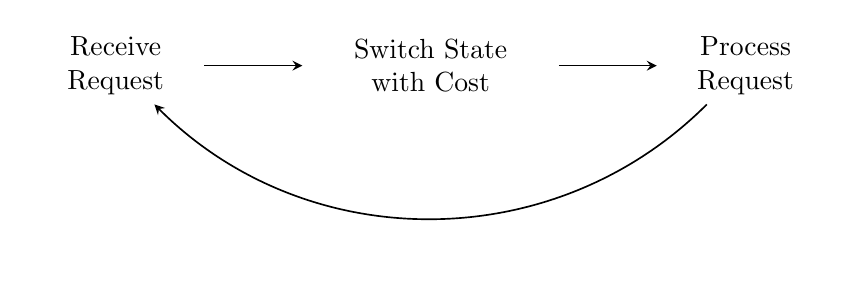
\begin{tikzpicture}[>=stealth, semithick]
            \node[align=center, text width=2cm] (0) at (0, 0) {Receive Request};
            \node[align=center, text width=3cm] (1) at (4, 0) {Switch State with Cost};
            \node[align=center, text width=2cm] (2) at (8, 0) {Process Request};
            \path[->] (0) edge (1)
                      (1) edge (2)
                      (2) edge[bend left=45] (0);
        \end{tikzpicture}
    \end{figure}

    \begin{definition}[{\cite[pp. 75-76]{Woeginger}}] \label{mts_definition}
        A \emph{Metrical Task System} (MTS) is a tuple \(((\mathcal{M}, d), \mathcal{T})\), where \((\mathcal{M}, d)\) is a finite metric space of cardinality \(N \coloneqq |\mathcal{M}|\), the \emph{set of states}, and \(\mathcal{T} \subseteq \left(\mathbb{R}_{\geq 0}^\infty\right)^N\) is the \emph{set of tasks}. If \(d(x, y) = 1\) for any \(x, y \in \mathcal{M}\) with \(x \neq y\), then the MTS is called \emph{uniform}.
    \end{definition}
    
    Given a fixed order of the elements in \(\mathcal{M}\), any task \(\tau \in \mathcal{T}\) can also be interpreted as a map of form \(\{0, 1, ..., N-1\} \to \mathbb{R}_{\geq 0}^\infty\), so we may write \(\tau(x)\) for \(x \in \mathcal{M}\). The term \(\tau(x)\) corresponds to the time to process the task \(\tau\) in the state \(x\). We will now also omit the term \(\mathcal{T}\), when specifying an MTS.

    \begin{figure}[!hbtp]
        \centering
        \begin{tikzpicture}[>=stealth, semithick]
            \node[align=center, text width=2cm] (0) at (0, 0) {\(\tau_i\)};
            \node[align=center, text width=3cm] (1) at (4, 0) {\((x_{i-1} \mapsto x_i)\) with cost \(x_{i-1}x_i\)};
            \node[align=center, text width=2cm] (2) at (8, 0) {\(\tau_i(x_i)\)};
            \path[->] (0) edge (1)
                      (1) edge (2)
                      (2) edge[bend left=45] (0);
        \end{tikzpicture}
    \end{figure}

    As we can see, the MTS model fits our description of how a system running an online algorithm behaves in theory. To get acquainted with \cref{mts_definition}, we shall describe three examples.

    \begin{example}[The Ice Cream Problem {\cite[pp. 74-75]{Woeginger}}]
        Suppose we work at an ice cream shop, which offers two flavors, vanilla (\(V\)) and strawberry (\(S\)). We can manually produce a gallon of vanilla ice cream at a cost of \(2\) and of strawberry ice cream at a cost of \(4\). The shop has an ice cream automaton, which can produce both flavors at half the cost each, but it can only produce gallons of one kind at a time (so either vanilla \(V_M\) or chocolate \(S_M\)) and needs to switch its mode at a cost of \(1\). The question is when to change the mode of the automaton to keep the cost low while serving customers. The following matrix captures these costs.
        \begin{align*}
            \begin{array}{c|c|c}
                    & V & S\\\hline
                V_M & 1 & 4\\
                S_M & 2 & 2
            \end{array}
        \end{align*}
        The MTS modelling this problem would be composed of the space \(\{V_M, S_M\}\) (in this order) of states with the metric \(d\colon (V_M, V_M) \mapsto 0, (V_M, S_M) \mapsto 1, (S_M, V_M) \mapsto 1, (S_M, S_M) \mapsto 0\) and the set of tasks \(\mathcal{T} \coloneqq \{(1, 4), (2, 2)\}\). The MTS is uniform.
    \end{example}

    \begin{example}[The Paging Problem {\cite[p. 124]{Borodin}}]
        Suppose we have an operating system that utilizes \emph{paging} to implement memory management. We have a large, slow memory of \(N \in \mathbb{N}\), \(N \geq 1\) pages and a small, fast memory of \(k \in \mathbb{N}\), \(1 \leq k \leq N\) pages. We can model the possible states of the smaller memory with a metric space \(\mathcal{M}\) of \(\binom{N}{k}\) elements, representing which \(k\) pages are currently in the small memory, assuming that the memory is filled at all times.

        \begin{figure}[!hbtp]
            \centering
            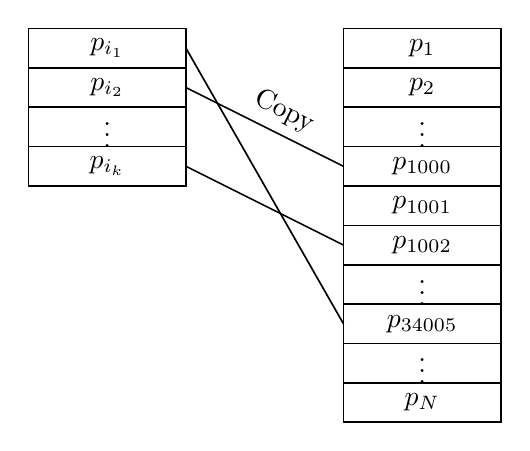
\begin{tikzpicture}[>=stealth, semithick]
                \draw (0, 0) rectangle (2, -0.5) node[pos=0.5] {\(p_{i_1}\)};
                \draw (0, -0.5) rectangle (2, -1) node[pos=0.5] {\(p_{i_2}\)};
                \draw (0, -1) rectangle (2, -1.5) node[pos=0.5] {\(\vdots\)};
                \draw (0, -1.5) rectangle (2, -2) node[pos=0.5] {\(p_{i_k}\)};
                \draw (4, 0) rectangle (6, -0.5) node[pos=0.5] {\(p_1\)};
                \draw (4, -0.5) rectangle (6, -1) node[pos=0.5] {\(p_2\)};
                \draw (4, -1.0) rectangle (6, -1.5) node[pos=0.5] {\(\vdots\)};
                \draw (4, -1.5) rectangle (6, -2.0) node[pos=0.5] {\(p_{1000}\)};
                \draw (4, -2.0) rectangle (6, -2.5) node[pos=0.5] {\(p_{1001}\)};
                \draw (4, -2.5) rectangle (6, -3.0) node[pos=0.5] {\(p_{1002}\)};
                \draw (4, -3.0) rectangle (6, -3.5) node[pos=0.5] {\(\vdots\)};
                \draw (4, -3.5) rectangle (6, -4.0) node[pos=0.5] {\(p_{34005}\)};
                \draw (4, -4.0) rectangle (6, -4.5) node[pos=0.5] {\(\vdots\)};
                \draw (4, -4.5) rectangle (6, -5.0) node[pos=0.5] {\(p_N\)};
                \draw (2, -0.25) -- (4, -3.75);
                \draw (2, -0.75) -- (4, -1.75) node[above, pos=0.56, rotate=-26.5651] {Copy};
                \draw (2, -1.75) -- (4, -2.75);
            \end{tikzpicture}
        \end{figure}
        
        In the figure, \(p_1, ..., p_N\) denote the pages and \(i_1, ..., i_k \in \mathbb{N}\), \(1 \leq i_1, ..., i_k \leq N\) denote pairwise different indices. Denoting the states by \(S_1, ..., S_{\binom{N}{k}}\), a suitable metric is \(d(S_i, S_j) \coloneqq k - |S_i \cap S_j|\), for which we can verify the properties of a metric, only the triangle inequality requires a case distinction. We now set \(\mathcal{T}\) as an \(N\)-set, for which every task \(\tau\) is associated with a page \(p\). As the task should output the page requested, we let
        \begin{align}
            \tau(S_i) \coloneqq \begin{cases}
                0 & p \in S_i\\
                \infty & p \notin S_i
            \end{cases}
        \end{align}
        for any \(i \in \mathbb{N}\), \(1 \leq i \leq \binom{N}{k}\) to force a suitable online algorithm to switch the state to one which contains the requested page. This MTS is not uniform for \(N > 3\) and \(k > 1\).
    \end{example}

    \begin{example}[The \(k\)-Server Problem {\cite[pp. 87-88]{Woeginger}}]
        We are given a metric space \(\mathcal{M}\) and \(k\) servers which reside on one point of the space each. A request for the entire system arrives at one of the points in the space, meaning that one of the servers needs to move to the point to serve the request. Wlog. we assume, that two or more servers can sit at the same point.

        \begin{figure}[!hbtp]
            \centering
            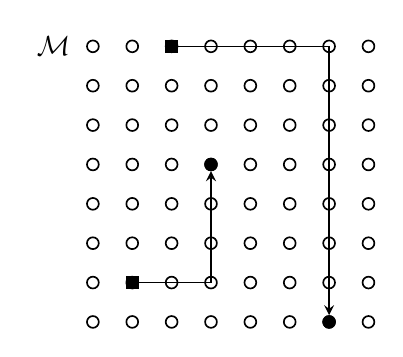
\begin{tikzpicture}[>=stealth, semithick]
                \tikzset{point/.style={draw, circle, inner sep=0pt, minimum size=1.5mm}}
                \newcommand{\dw}{0.5}
                \foreach \x in {0, 1, ..., 7} {
                    \foreach \y in {0, 1, ..., 7} {
                        \node[point] at (\dw*\x, \dw*\y) {};
                    }
                }
                \node at (-0.5, \dw * 7) {\(\mathcal{M}\)};
                \node[fill, point] (r1) at (\dw*3, \dw*4) {};
                \node[fill, point] (r2) at (\dw*6, \dw*0) {};
                \node[fill, point, rectangle] (k1) at (\dw*1, \dw*1) {};
                \node[fill, point, rectangle] (k2) at (\dw*2, \dw*7) {};
                \draw[->] (k1) -- (\dw*3, \dw*1) -- (r1);
                \draw[->] (k2) -- (\dw*6, \dw*7) -- (r2);
            \end{tikzpicture}
        \end{figure}

        A suitable formulation as an MTS would be to equip \(\mathcal{M}^k\) with the metric assigning two configurations the minimum distance the servers need to travel from one configuration starting to cover the same points in the same weights as in the other configuration, also called the \emph{configuration distance} of two \emph{configurations}, i.e. states. To each task \(\tau\) we then have a point \(x \in \mathcal{M}\) associated, s.t. \(\tau(x_1, ..., x_k) = 0\), iff \(x = x_i\) for an \(i \in \mathbb{N}\), \(1 \leq i \leq k\). Otherwise \(\tau(x_1, ..., x_k) = \infty\).
    \end{example}

    \paragraph{\textbf{Online Algorithms}} With the definition of an MTS, we can now especially formulate the concept of an online algorithm in the MTS model, as well as the optimal algorithm and competitiveness. For the following paragraphs, let \(\mathcal{M}\) denote an MTS, \(x_0 \in \mathcal{M}\) an initial state and \(\tau \in \mathcal{T}^n\), \(n \in \mathbb{N}\), be a one-indexed sequence of tasks.

    \begin{definition}[{\cite[p. 76]{Woeginger}}]
        Let \(x \in \mathcal{M}^n\) be a one-indexed sequence of states. Set
        \begin{align}
            \text{cost}(x_0, \tau, x) &\coloneqq \sum_{i=1}^n x_{i-1}x_i + \tau_i(x_i)\\
            \text{opt}(x_0, \tau) &\coloneqq \min_{x' \in \mathcal{M}^n} \text{cost}(x_0, \tau, x')
        \end{align}
        as the cost of processing the task sequence \(\tau\) under the state sequence \(x\) and the optimal cost respectively. Let further \(\mathcal{T}^* \coloneqq \bigcup_{m=1}^\infty \mathcal{T}^m\). A (deterministic) \emph{online strategy/online algorithm} for \(\mathcal{M}\) is a map \(\mathcal{A}\colon \mathcal{M} \times \mathcal{T}^* \to \mathcal{M}\). We further set the cost of execution by \(\mathcal{A}\) as
        \begin{align}
            \text{cost}_{\mathcal{A}}(x_0, \tau) \coloneqq \text{cost}(x_0, \tau, \mathcal{A}(x_0, \tau_1)\mathcal{A}(x_0, \tau_1\tau_2)...\mathcal{A}(x_0, \tau_1\tau_2...\tau_n))
        \end{align}
        \(\mathcal{A}\) is called \emph{\(c\)-competitive with initial function \(\alpha\colon \mathcal{M} \to \mathcal{R}\)}, where \(c \in \mathbb{R}\), if for any \(x_0 \in \mathcal{M}\) and \(\tau \in \mathcal{T}^*\), we have
        \begin{align}
            \text{cost}_{\mathcal{A}}(x_0, \tau) \leq c \; \text{opt}(x_0, \tau) + \alpha(x_0)
        \end{align}
        Furthermore, the value \(\text{argmin}_{c \in \mathbb{R}} (\mathcal{A} \text{ is } c \text{-competitive})\), if it exists, is called the \emph{competitive-ratio} of \(\mathcal{A}\).
    \end{definition}

    The definitions from the model correspond to the same definition of competitiveness as discussed in class, which hints at the abstractions made being well-chosen. As mentioned, this is the definition for deterministic online algorithms. At the end, we will mention a few different models.

    \phantom{}

    \paragraph{\textbf{The Work Function Algorithm}}

    In this part, we will give an optimal competitive algorithm for an arbitrary MTS with the competitive ratio only depending on \(N\), the so-called \emph{Work Function Algorithm} (WFA). We first need to define what \emph{work functions} are.

    \begin{definition}[Work Functions]
        The function
        \begin{align}
            \omega\colon \mathcal{M} \to \mathbb{R}, x \mapsto \textstyle\min_{(x_1, ..., x_{n-1}) \in \mathcal{M}^{n-1}} \text{cost}(x_0, \tau, (x_0, x_1, ..., x_{n-1}, x))
        \end{align}
        is called the \emph{work function} for \(x_0\) and \(\tau\).
    \end{definition}

    The work function describes the minimal cost for reaching a given state \(x\) after processing \(\tau\). The work function can be computed using a dynamical program. Let \(\omega_i\) for any \(i \in \mathbb{N}\), \(0 \leq i \leq n\), denote the work function of \(x_0\) and \((\tau_1, ..., \tau_i)\) computing the lowest costs for the first \(i\) tasks. Then
    \begin{align}
        \omega_0(x) &= x_0x\\
        \omega_{i+1}(x) &= \min_{x' \in \mathcal{M}} \omega_i(x') + \tau_{i+1}(x') + x'x \label{work_function_comp_dyn_prog_second_stmt}
    \end{align}
    We can verify the correctness through induction: The base formula for \(\omega_0\) is clear. Then the lowest cost for computing the value of \(\omega_{i+1}\) is given by the above term and is also optimal by the induction assumption.

    The work function and our ability to compute it now allows the formulation of the so-called \emph{Work Function Algorithm}. In the same manner as the formal definition we describe it as the function \(\text{WFA}\colon \mathcal{M} \times \mathcal{T}^* \to \mathcal{M}\).

    \phantom{}

    \begin{mdframed}
        \paragraph*{\textbf{The Work Function Algorithm (WFA)}} Let \(i \in \mathbb{N}\), \(1 \leq i \leq n-1\) and suppose the states \(x_0, x_1, ..., x_i\) have already been computed. Then the WFA chooses the next state by
        \begin{align*}
            x_{i+1} &\in \arg\min_{x \in \mathcal{M}} \omega_{i+1}(x)+x_ix \tag{\(\dagger\)} \label{wfa_first_condition}\\
            \text{s.t. } \omega_{i+1}(x_{i+1}) &= \omega_i(x_{i+1})+\tau_{i+1}(x_{i+1}) \tag{\Ankh} \label{wfa_second_condition}
        \end{align*}
    \end{mdframed}

    \phantom{}

    This algorithm was first suggested by Ricklin, based on results by Borodin, Linial and Saks \cite[p. 123, p. 132]{Borodin}. A rough interpretation may be, that the algorithm chooses the next state by minimizing the cost to process \((\tau_1, ..., \tau_{i+1})\) and to move from \(x_i\) to \(x_{i+1}\). The second condition also establishes, that in the state \(x_{i+1}\), we process \(\tau_{i+1}\). It is not clear why it is optimal, nor why it is well-defined, which is the first question we are going to tackle.

    \begin{theorem}[{\cite[pp. 132-133]{Borodin}}]
        The WFA is well-defined.
    \end{theorem}

    \begin{proof}
        As \(\mathcal{M}\) is finite, there is always an element sufficing (\ref{wfa_first_condition}). We first prove the direction \((\leq)\) for any such element and then prove the existence of one sufficing \((\geq)\) for (\ref{wfa_second_condition}).

        \((\leq)\) Notice, that for any \(x \in \mathcal{M}\), we have from the definition of the work function, that
        \begin{align}
            \underbrace{\omega_{i+1}(x)}_{\begin{array}{c}\text{Optimal cost for processing }\\ (\tau_1, ..., \tau_{i+1}) \text{ and ending in } x\text{.}\end{array}} \leq \underbrace{\omega_i(x) + \tau_{i+1}(x)}_{\begin{array}{c}\text{Optimal cost for processing } (\tau_1, ..., \tau_i) \text{,}\\\text{ending in } x \text{ and then processing } \tau_{i+1} \text{ there.}\end{array}} \label{wfa_well_def_first_direction}
        \end{align}
        \((\geq)\) Let
        \begin{align}
            x' &\in \arg\min_{x \in \mathcal{M}} \omega_{i+1}(x) + x_ix\\
            x^* &\in \arg\min_{x \in \mathcal{M}} \omega_i(x)+\tau_{i+1}(x)+xx' \label{x_star_def}
        \end{align}
        These elements give the minimas from (\ref{wfa_first_condition}) and (\ref{work_function_comp_dyn_prog_second_stmt}), where the latter is applied on \(x'\). We claim
        \begin{align}
            \omega_{i+1}(x^*) + x_ix^* \leq \omega_{i+1}(x') + x_ix' \label{wfa_well_def_helper_claim}
        \end{align}
        For that, we have the three inequalities
        \begin{align}
            \omega_{i+1}(x^*)+x^*x_i &\leq \omega_i(x^*)+\tau_{i+1}(x^*)+x^*x_i \label{wfa_well_def_proof_ineq_1}\\
            \omega_i(x^*)+\tau_{i+1}(x^*) + x^*x_i &= \omega_{i+1}(x') + x^*x_i - x^*x' \label{wfa_well_def_proof_ineq_2}\\
            x^*x_i - x^*x' &\leq x'x_i \label{wfa_well_def_proof_ineq_3}
        \end{align}
        We obtain (\ref{wfa_well_def_proof_ineq_1}) by taking (\ref{wfa_well_def_first_direction}) for \(x = x^*\) and adding \(x^*x_i\). (\ref{wfa_well_def_proof_ineq_2}) is obtained by taking the statement in (\ref{x_star_def}) and adding \(x^*x_i-x^*x'\). (\ref{wfa_well_def_proof_ineq_3}) is then obtained by the triangle inequality of the metric. Combining all three statements by following the equalities and inequalities from left to right, top to bottom, we obtain the statement. By that, we first have that \(x^*\) satisfies (\ref{wfa_first_condition}), as \(x'\) minimizes the term involved, additionally giving that our claim is an equality. \((\geq)\) now follows from
        \begin{align}
            \omega_{i+1}(x^*)+x^*x_i &\overset{\ref{wfa_well_def_helper_stmt_1}}{=} \omega_{i+1}(x')+x'x_i \overset{\ref{wfa_well_def_helper_stmt_2}}{=} \omega_i(x^*)+\tau_{i+1}(x^*)+x'x^*+x'x_i \overset{\ref{wfa_well_def_helper_stmt_3}}{\leq} \omega_i(x^*)+\tau_{i+1}(x^*)+x^*x_i
        \end{align}
        \begin{enumerate}[label=(\arabic*)]
            \item Using that (\ref{wfa_well_def_helper_claim}) is an equality. \label{wfa_well_def_helper_stmt_1} 
            \item Due to (\ref{x_star_def}). \label{wfa_well_def_helper_stmt_2}
            \item By the triangle inequality. \label{wfa_well_def_helper_stmt_3}
        \end{enumerate}
        giving the statement.
    \end{proof}

    We now analyze the competitiveness of the WFA. For that, we will require the following lemma.

    \begin{theorem}[{\cite[pp. 133-134]{Borodin}}] \label{wfa_competitiveness_theorem}
        For any \(i \in \mathbb{N}\), \(0 \leq i \leq n\), we have
        \begin{align}
            \text{cost}_{\text{WFA}}(x_0, (\tau_1, ..., \tau_i)) + B_0 \leq B_i \leq (2N-1) \; \text{opt}(x_0, (\tau_1, ..., \tau_i)) + (2N-2) \mu
        \end{align}
        where \((x_1, ..., x_n) \in \mathcal{M}^n\) is the sequence of states produced by the WFA and
        \begin{align}
            \mu \coloneqq \max_{x, x' \in \mathcal{M}} xx' \text{, } B_i \coloneqq 2\sum_{x \in \mathcal{M} \setminus \{x_i\}} \omega_i(x) + \omega_i(x_i)
        \end{align}
        In other words, the WFA is \((2N-1)\)-competitive.
    \end{theorem}

    \begin{proof}
        We start by proving the first inequality. By (\ref{wfa_first_condition}),
        \begin{align}
            \omega_{i+1}(x_{i+1})+x_ix_{i+1} = \min_{x \in \mathcal{M}} \omega_{i+1}(x)+x_ix \leq \omega_{i+1}(x_i) + x_ix_i = \omega_{i+1}(x_i)
        \end{align}
        And by (\ref{wfa_second_condition}), \(\omega_{i+1}(x_{i+1})-\omega_i(x_{i+1}) = \tau_{i+1}(x_{i+1})\). Reordering the first result and plugging in the second, we have
        \begin{align}
            \omega_{i+1}(x_i)-\omega_i(x_{i+1}) \geq x_ix_{i+1} + \tau_{i+1}(x_{i+1})
        \end{align}
        We claim \(B_{i+1} - B_i \geq \omega_{i+1}(x_i)-\omega_i(x_{i+1})\). First, notice that \(\omega_i\) is monotonely increasing wrt. \(i\), as by (\ref{work_function_comp_dyn_prog_second_stmt}), we have for any \(x \in \mathcal{M}\)
        \begin{align}
            \omega_{i+1}(x) = \min_{x' \in S} \omega_i(x')+\tau_{i+1}(x') + x'x \geq \omega_i(x)
        \end{align}
        So
        \begin{align}
            B_{i+1}-B_i &= 2 \left(\sum_{x \in \mathcal{M} \setminus \{x_i, x_{i+1}\}} \underbrace{\omega_{i+1}(x)-\omega_{i}(x)}_{\geq 0}\right)\\
            &\phantom{\geq}+ \underbrace{\omega_{i+1}(x_{i+1}) - \omega_{i}(x_{i+1})}_{\geq 0} + \underbrace{\omega_{i+1}(x_i) - \omega_{i}(x_i)}_{\geq 0} + (\omega_{i+1}(x_i) - \omega_i(x_{i+1}))
        \end{align}
        This gives the claim. Especially, we now have \(B_{i+1}-B_i \geq x_ix_{i+1}+\tau_{i+1}(x_{i+1})\), giving the telescope sum
        \begin{align}
            \text{cost}_{\text{WFA}}(x_0, (\tau_1, ..., \tau_i)) = \sum_{j=1}^i x_{j-1}x_j + \tau_j(x_j) \leq \sum_{j=1}^i B_j-B_{j-1} = B_i - B_0
        \end{align}
        and by that giving the first inequality.

        For the second inequality, observe from the definition, that \(\omega_i(x) = \min_{x' \in \mathcal{M}} \omega_i(x') + x'x \leq \min_{x' \in \mathcal{M}} \omega_i(x') + \mu\). There is further at least one end state giving the optimum cost, s.t. plugging that in gives
        \begin{align}
            B_i = 2\sum_{x \in \mathcal{M} \setminus \{x_i\}} \omega_i(x) + \omega_i(x_i) \leq (2N-2) (\text{opt}(x_0, (\tau_1, ..., \tau_i)) + \mu) + \text{opt}(x_0, (\tau_1, ..., \tau_i))
        \end{align}
    \end{proof}

    Lastly, we can establish that \((2N-1)\) is also the competitive ratio of the WFA, but we are going to omit that here. The following theorem only presents this result for general deterministic online algorithms.

    \begin{theorem}[{\cite[pp. 128-132]{Borodin}}]
        The competitive ratio of any deterministic online algorithm for general MTS is lower bounded by \((2N-1)\).
    \end{theorem}

    One last remark: As we can observe, the WFA runs in time \(O(n N^2)\). A runtime of \(O(n N^2)\) is required to compute the first \(n\) work functions, for which the algorithm needs to compute \(N\) values each taking minimums over the \(N\) states. Each of the \(n\) algorithm states then requires checking all \(N\) values of a work function.

    \phantom{}

    \paragraph{\textbf{Results on WFAs for Some Problems}}

    The following table gives an overview of results on the initial examples, as well as the different versions of the \(k\)-server problem. The values \(c_{\text{WFA}}\) and \(c_{\text{Better}}\) shall denote the competitiveness of the associated WFA and some better known algorithms. We know the first two examples already. Especially for the \(k\)-server problem however, there are multiple results on different restrictions of the problem, illustrating the richness of that problem. Especially, the following conjecture, still open after much effort, exist.

    \begin{conjecture}[{\cite[pp. 152-153]{Borodin}}]
        There exists a \(k\)-competitive deterministic online algorithm for the \(k\)-server algorithm over any metric space.
    \end{conjecture}

    \begin{table}[!hbtp]
        \begin{tabular}{c|c|c}
            Problem & \(c_{\text{WFA}}\) & \(c_{\text{Better}}\)\\\hline
            Ice Cream & \(3\) & \(7/6\) (claim in exercise, \cite[pp. 80-82]{Woeginger}) \\
            Paging & \(2\binom{N}{k}-1\) & \(k\) (tight, \cite[pp. 54-56]{Woeginger})\\
            \(k\)-Server MTS WFA & \(2N^k-1\) & See below\\
            \(2\)-Server WFA & \(2\) (tight, \cite[pp. 87-89, p. 94]{Woeginger}) & None\\
            \(k\)-Server WFA, \(k \geq 3\) & \(2k-1\) (\cite[pp. 92-93]{Woeginger}) & Open\\
            \(k\)-Server WFA, \(|\mathcal{M}| = k+2\) & \(k\) (tight, \cite[pp. 87-89, pp. 94-95]{Woeginger}) & None
        \end{tabular}
    \end{table}

    Especially the example of paging shows how weak the WFA can be in comparison to other online algorithms, but the generality still allows to prove the existence of a competitive algorithm for an any online algorithmic problem, no matter how difficult, if it can be expressed as an MTS. Especially, in the case of algorithms for the \(k\)-server problem, it can lead to conjectured nearly optimal algorithms.

    \printbibliography{}
\end{document}
